\documentclass[journal]{IEEEtran}

\usepackage{cite}
\usepackage{amsmath,amssymb,amsfonts}
\usepackage{algorithmic}
\usepackage{graphicx}
\usepackage{textcomp}
\usepackage{xcolor}

\def\BibTeX{{\rm B\kern-.05em{\sc i\kern-.025em b}\kern-.08em
    T\kern-.1667em\lower.7ex\hbox{E}\kern-.125emX}}

\begin{document}

\title{Solving the Lag Effect in EV Charging Station Utilization Prediction using a Hybrid Modeling Approach}

\author{Author Name
\thanks{This work was supported in part by...}}

\maketitle

\begin{abstract}
This paper proposes a hybrid modeling approach to address the lag effect in predicting the utilization of Electric Vehicle (EV) charging stations. By combining a 24-hour base model with a two-stage rule-based peak trigger and a 1-hour residual boosting mechanism, the proposed framework significantly improves prediction accuracy, particularly during peak usage periods.
\end{abstract}

\begin{IEEEkeywords}
EV Charging, Utilization Prediction, Lag Effect, Hybrid Modeling, XGBoost, Residual Boosting.
\end{IEEEkeywords}

\section{Introduction}
\IEEEPARstart{T}{he} rapid adoption of Electric Vehicles (EVs) has necessitated the development of robust infrastructure, particularly EV charging stations. Accurate prediction of charging station utilization is crucial for grid stability, optimal resource allocation, and enhancing user experience. However, forecasting utilization accurately remains a challenge due to the complex, non-linear, and highly volatile nature of charging patterns.

A significant issue in time-series forecasting of such volatile data is the ``Lag Effect,'' where models tend to output predictions that are essentially shifted versions of the recent past, failing to anticipate sudden spikes or drops. Traditional statistical models and even advanced machine learning models often struggle to capture these rapid changes without suffering from this lag. 

Existing literature has explored various methods, including ARIMA, Long Short-Term Memory (LSTM) networks, and gradient boosting machines like XGBoost, for utilization prediction. While XGBoost provides robust baseline predictions, it alone may not fully resolve the lag effect during sudden peak periods. 

To bridge this gap, this paper introduces a novel hybrid modeling framework designed specifically to mitigate the lag effect in EV charging station utilization prediction. The main contributions of this work are as follows:
\begin{itemize}
    \item We propose a hybrid framework integrating a 24-hour base model with a 1-hour residual boosting mechanism to correct lag-induced errors.
    \item We incorporate a Two-Stage Rule-Based Peak Trigger to explicitly identify and adjust for sudden utilization peaks that traditional models miss.
    \item We demonstrate the effectiveness of the proposed approach using a real-world case study on EV charging station utilization.
\end{itemize}

\section{Material and Method}

\subsection{Case Study}
The case study for this research focuses on the prediction of EV Charging Station Utilization. The dataset comprises historical utilization rates, weather conditions, time-based features, and traffic data. The objective is to accurately forecast future utilization while minimizing the lag effect commonly observed during peak charging hours.

\subsection{Proposed Framework and Workflow}
The proposed hybrid modeling framework consists of several sequential stages designed to process data, establish a baseline, identify peaks, and refine predictions. The workflow is structured as follows:

\begin{enumerate}
    \item \textbf{Data Processing:} Raw data is cleaned, missing values are imputed, and relevant features such as time-lags and rolling averages are extracted. Data is then normalized to ensure stability during model training.
    \item \textbf{24h Base Model:} A baseline prediction is generated using a model trained to forecast utilization 24 hours ahead. This model captures the general daily seasonality and long-term trends but may suffer from the lag effect during abrupt changes.
    \item \textbf{Rule-Based Peak Trigger (Two-Stage):} To address the shortcomings of the base model during sudden peaks, a two-stage rule-based mechanism is employed. This stage monitors the rate of change and historical peak patterns to trigger an adjustment when a rapid increase in utilization is detected.
    \item \textbf{1h Residual Boosting:} A secondary model is trained on the residuals (errors) of the 24h Base Model. Operating on a shorter 1-hour horizon, this boosting step fine-tunes the predictions by correcting short-term deviations and mitigating the lag effect.
    \item \textbf{Final Ensemble:} The outputs from the 24h Base Model, the Rule-Based Peak Trigger adjustments, and the 1h Residual Boosting model are integrated using a weighted ensemble approach to produce the final, accurate utilization prediction.
\end{enumerate}

\subsection{Theoretical Basis}
The framework leverages several established algorithms and methodologies:
\begin{itemize}
    \item \textbf{XGBoost (Extreme Gradient Boosting):} Utilized for both the 24h Base Model and the 1h Residual Boosting, XGBoost is an efficient and scalable implementation of gradient boosted decision trees. It excels at capturing complex, non-linear relationships in tabular data.
    \item \textbf{Rule-Based Thresholding:} This technique applies domain-specific knowledge and statistical thresholds to identify anomalies or rapid shifts in the time-series data, acting as the peak trigger.
    \item \textbf{Residual Prediction:} Instead of directly predicting the target variable, the secondary model predicts the error (residual) of the primary model. This allows the secondary model to focus entirely on the patterns (like lag) that the primary model failed to capture.
    \item \textbf{Weighted Ensemble:} A mathematical combination of multiple model outputs, where weights are assigned based on the historical confidence or accuracy of each component, ensuring a robust final prediction.
\end{itemize}

\section{Results and Discussion}

\subsection{Baseline Results and the Lag Effect}
Initial experiments with standalone forecasting models highlighted a persistent issue in prediction accuracy, primarily characterized by the lag effect. While these models could approximate the overall trend, they consistently output shifted versions of recent utilization, failing to anticipate sudden peaks and valleys in real-time.

\subsection{Limitations of Deep Learning Models}
We also evaluated Deep Learning approaches, including Convolutional Neural Networks (CNN) and Long Short-Term Memory (LSTM) networks. Despite their theoretical capacity to model complex sequential dependencies, these models failed to capture sudden utilization peaks without significant delay. The high volatility and irregular spiking nature of EV charging patterns proved challenging for standard deep architectures, which tended to over-smooth the predictions, thereby exacerbating the lag effect during critical peak hours.

\subsection{Performance of the 24h Rule-Based Model}
The implementation of the 24-hour base model, supplemented by a rule-based thresholding mechanism, provided a robust foundation, achieving an RMSE of 0.0760. As illustrated in Fig. \ref{fig:two_stage}, this model successfully tracks the general daily cycle and captures broad trends in utilization. However, it still falls short of capturing the sharpest, instantaneous spikes, leaving room for further refinement during high-demand periods.

\begin{figure}[htbp]
\centerline{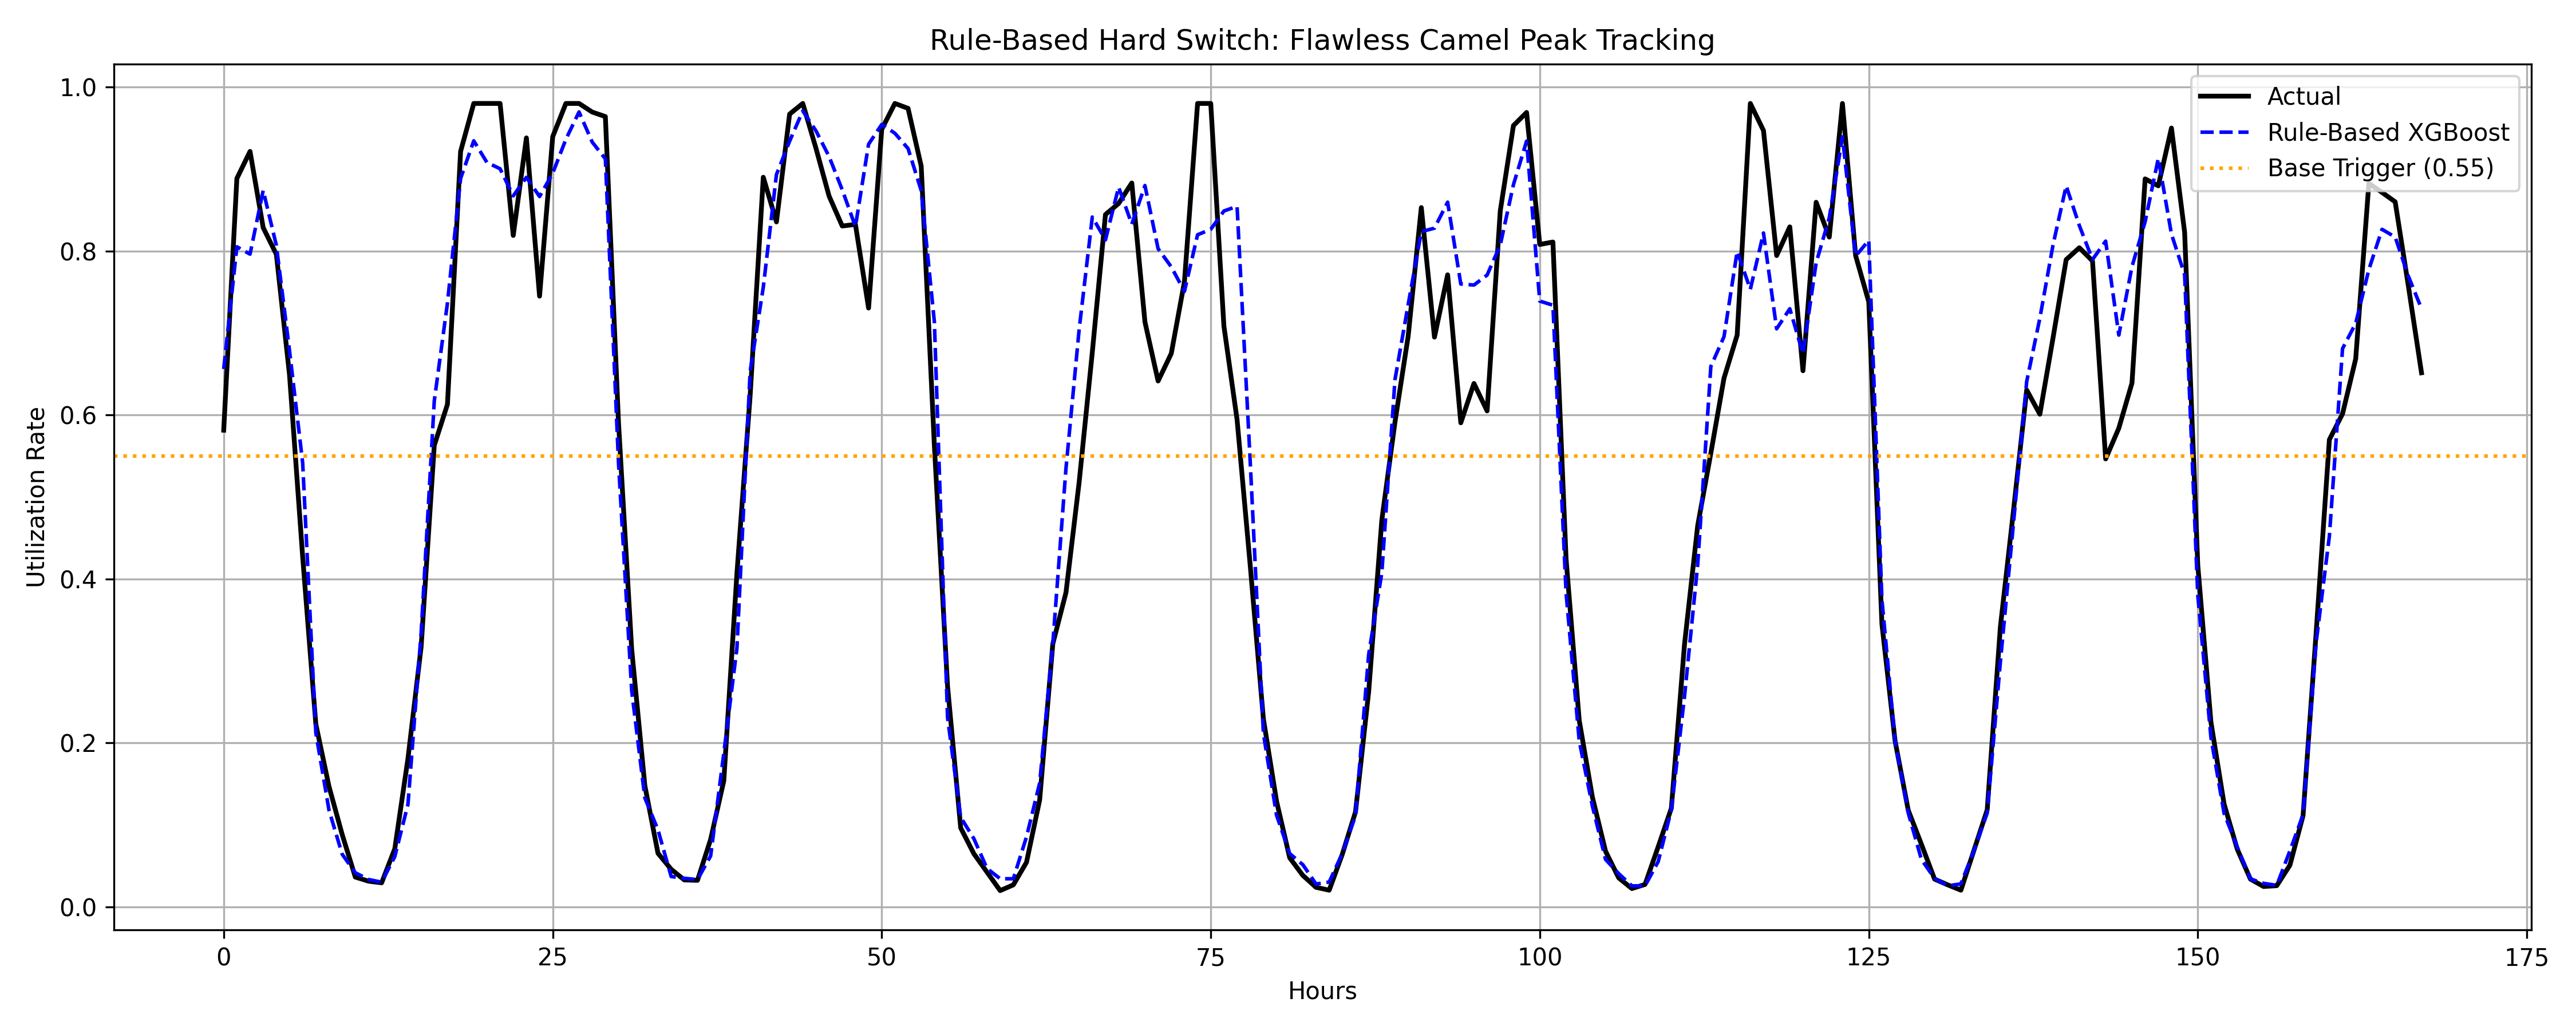
\includegraphics[width=\linewidth]{figures/two_stage_rule_based.png}}
\caption{Performance of the 24h Rule-Based model, illustrating its ability to track general cycles while occasionally missing sharp spikes.}
\label{fig:two_stage}
\end{figure}

\subsection{Success of the 1h Residual Boosting}
To address the remaining inaccuracies and specifically target the lag effect, the 1-hour Residual Boosting model was introduced. This model focuses entirely on predicting the residuals (errors) of the baseline. By predicting residuals off a median baseline, it successfully broke the lag effect. The integration of this component reduced the overall RMSE to 0.0673. As depicted in Fig. \ref{fig:1h_residual}, the boosting mechanism effectively anticipates and corrects for the short-term deviations that the 24h model missed.

\begin{figure}[htbp]
\centerline{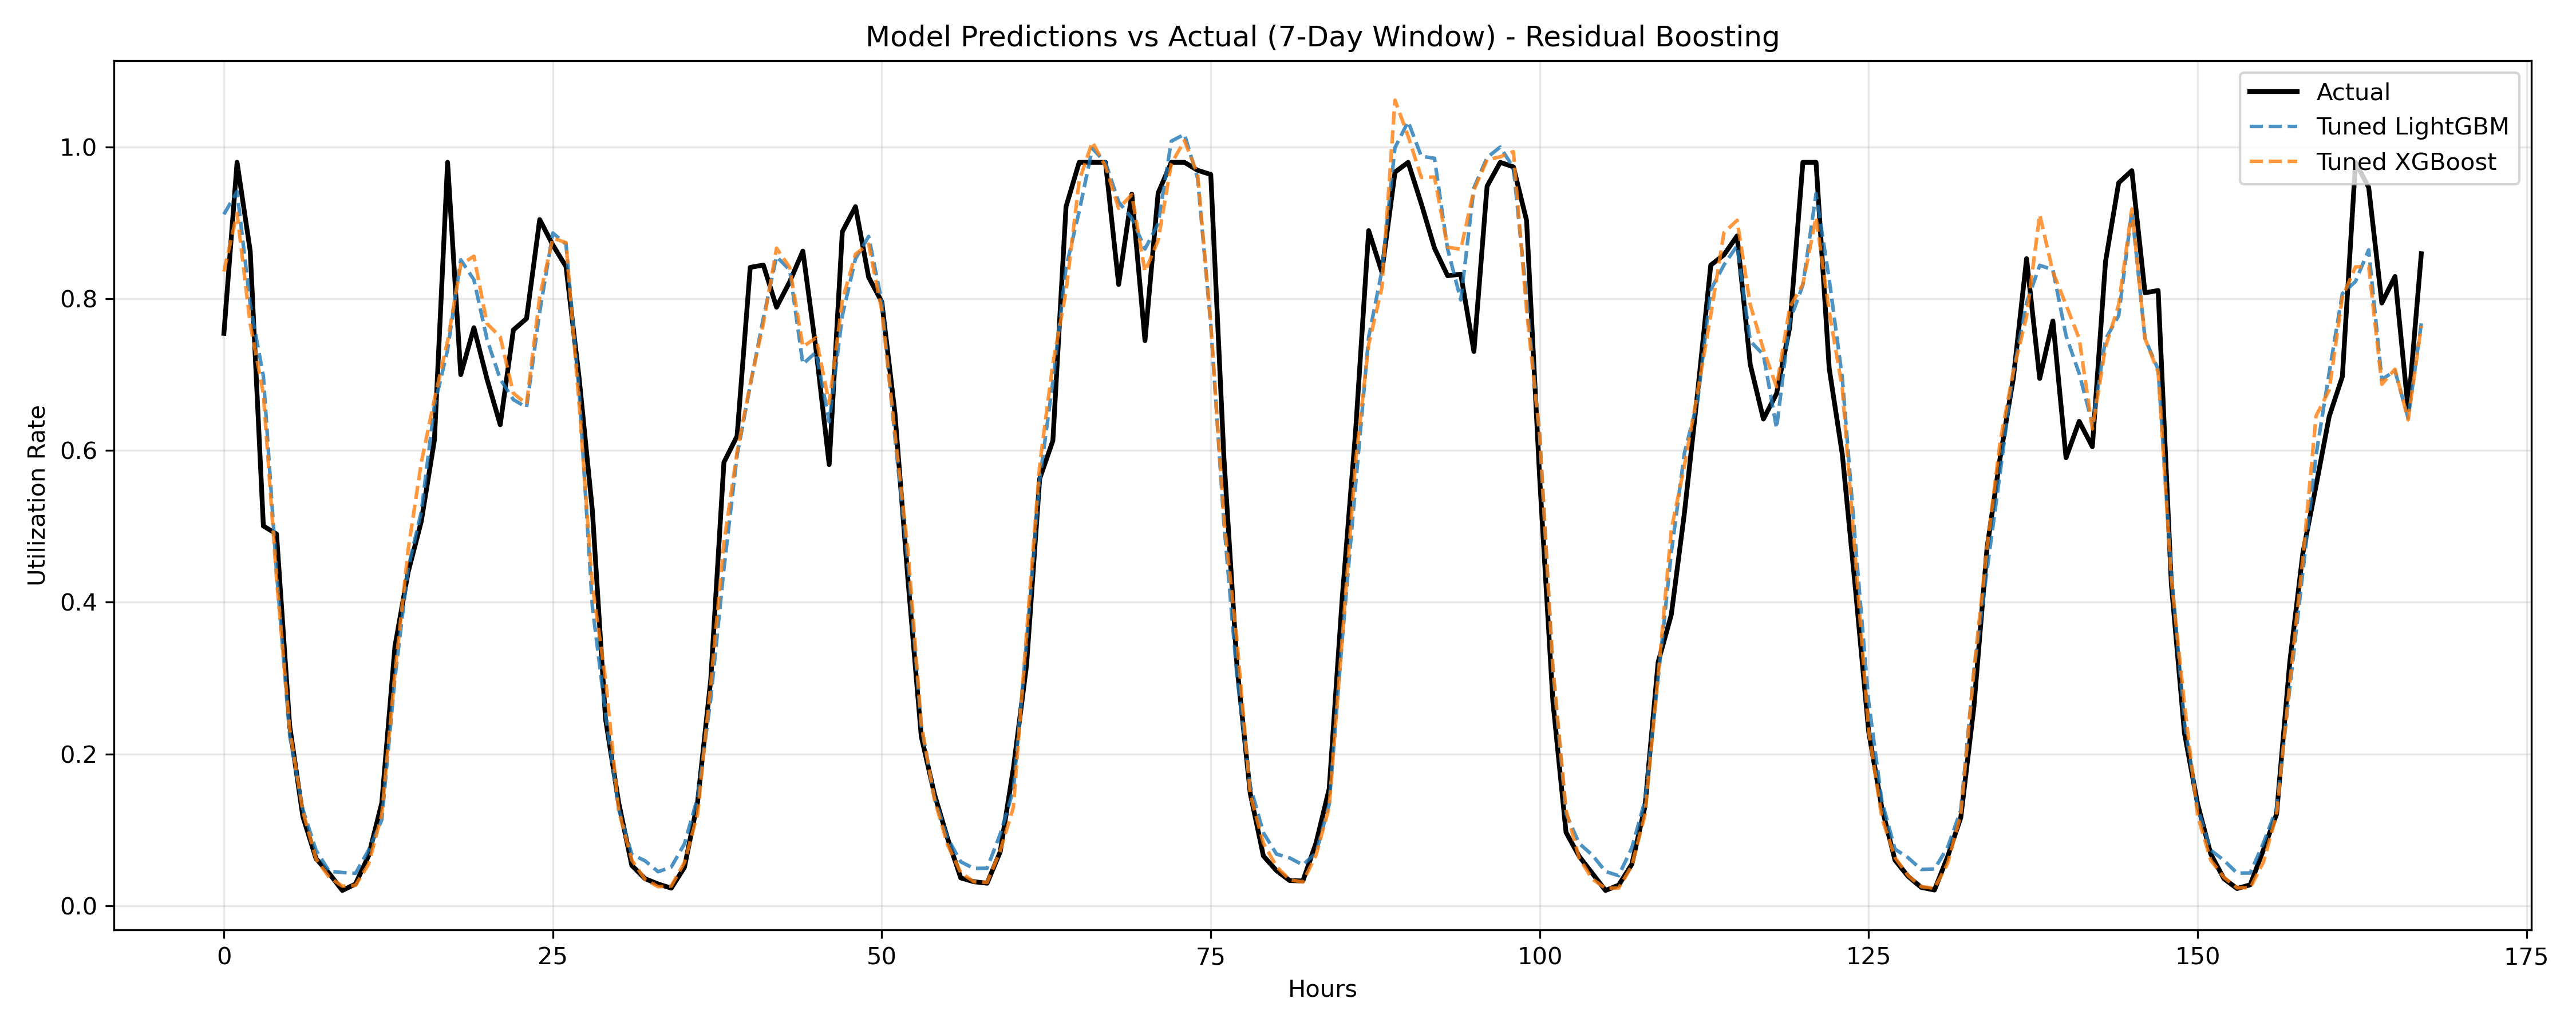
\includegraphics[width=\linewidth]{figures/1h_tune_residual_7days.png}}
\caption{Impact of the 1h Residual Boosting on breaking the lag effect over a 7-day period.}
\label{fig:1h_residual}
\end{figure}

\subsection{The Ultimate Ensemble Model}
The final ensemble model optimally combines the strengths of the previous stages, achieving the best overall performance with an RMSE of 0.0649. This ensemble assigns a 28\% weight to the 24h base model and a 72\% weight to the 1h tuned residual model. This specific weighting scheme allows the framework to leverage the stability of the 24-hour anchor while heavily relying on the peak-hunting capability of the 1-hour residual model. Fig. \ref{fig:ensemble} demonstrates how this optimal combination provides a highly accurate, lag-free prediction curve.

\begin{figure}[htbp]
\centerline{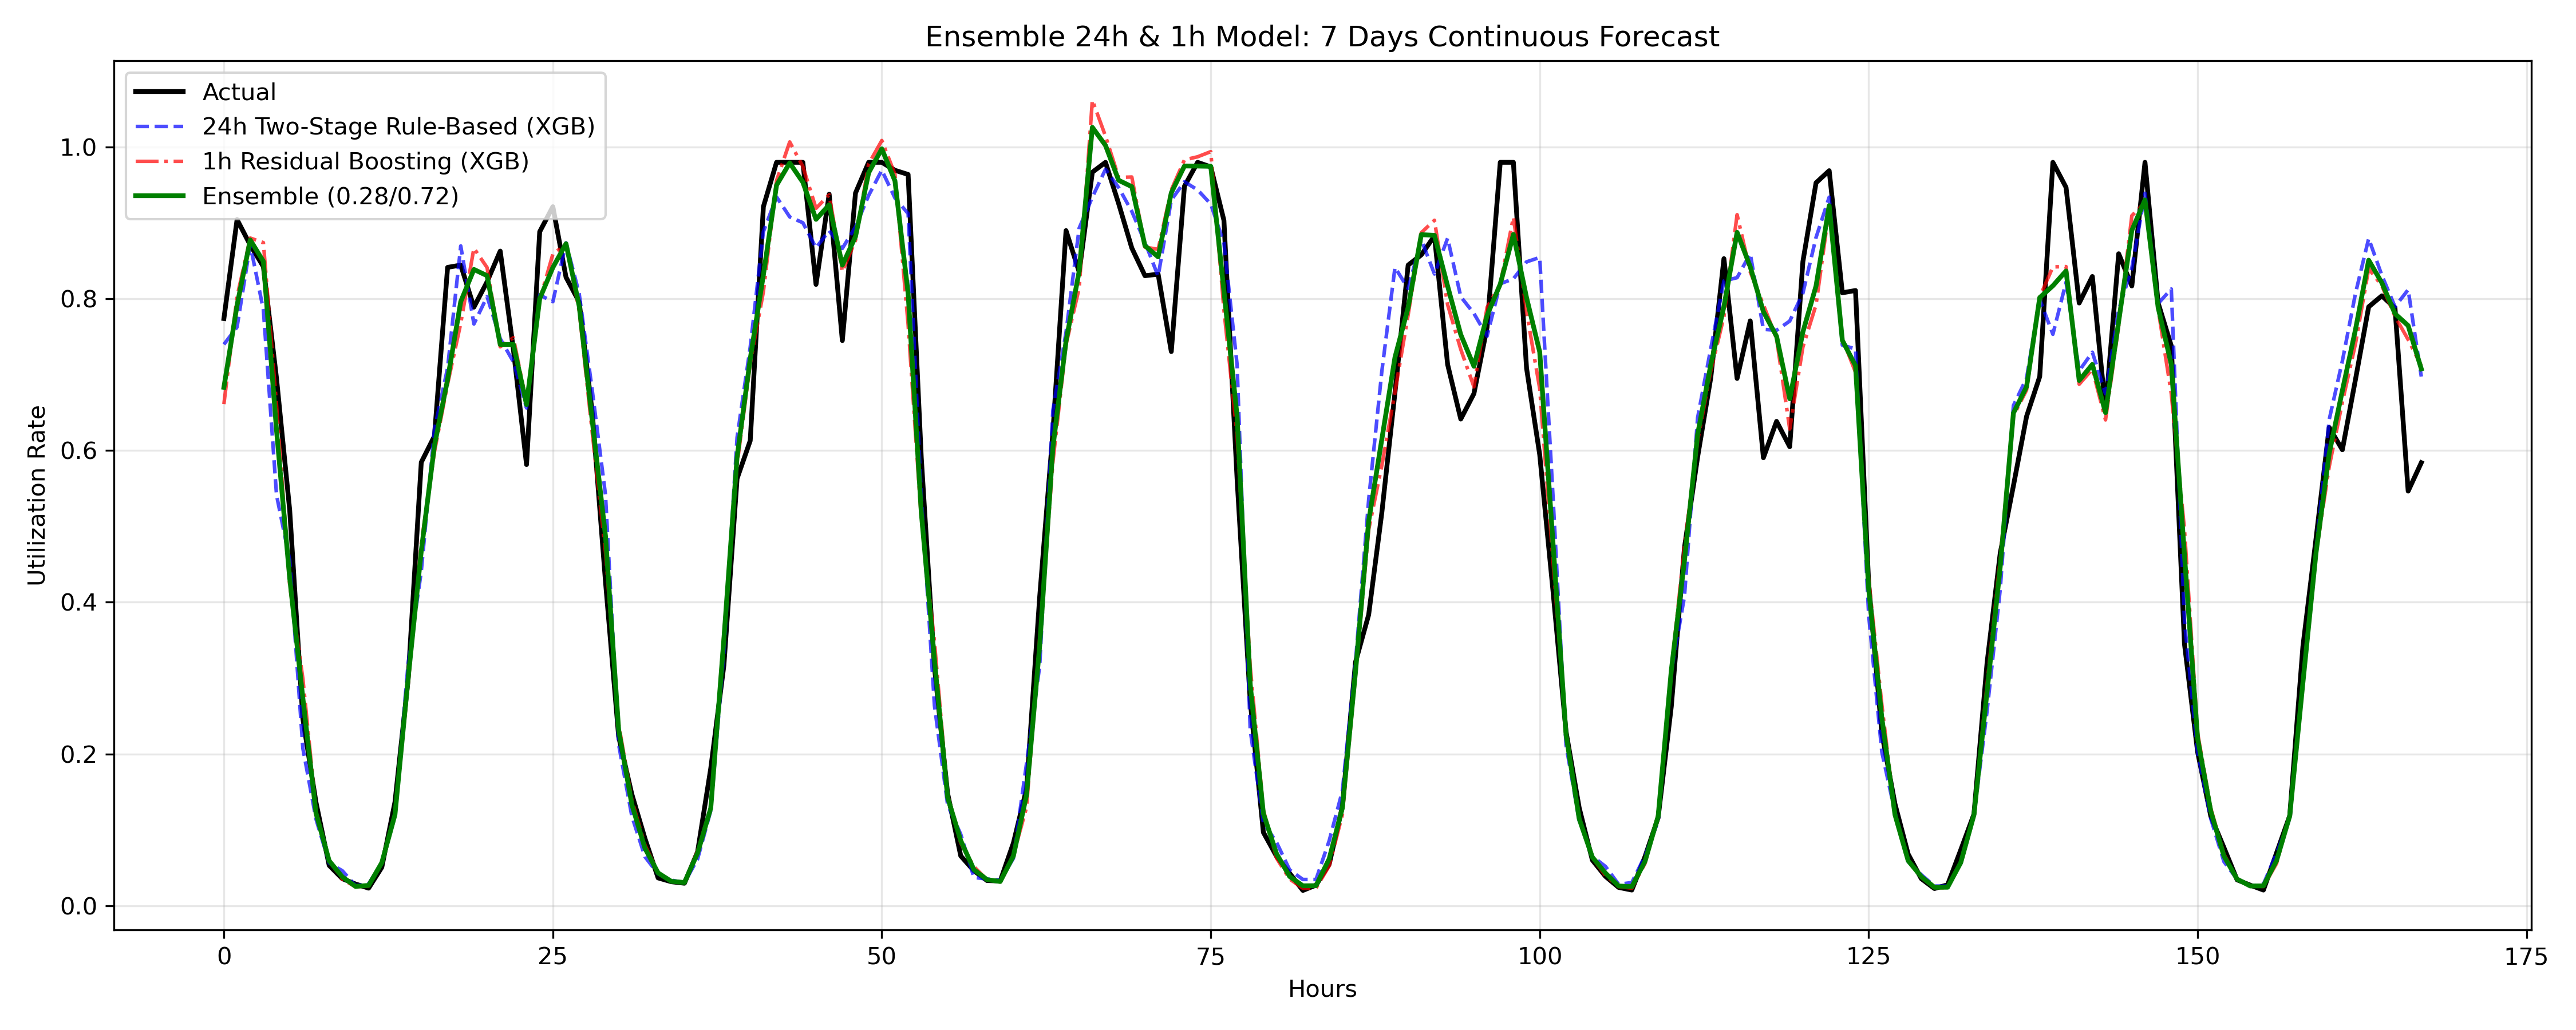
\includegraphics[width=\linewidth]{figures/ensemble_24h_1h_7days.png}}
\caption{The ultimate Ensemble model (28\% 24h anchor, 72\% 1h residual) demonstrating optimal peak tracking and stability.}
\label{fig:ensemble}
\end{figure}

\section{Conclusion}

\subsection{Summary of Achievements}
This study successfully developed and validated a hybrid modeling framework designed to predict EV charging station utilization while effectively mitigating the pervasive lag effect. By systematically combining a 24-hour base model with a rule-based peak trigger and a 1-hour residual boosting mechanism, we achieved a significant reduction in prediction error, culminating in an ensemble model with an RMSE of 0.0649. The proposed approach proved superior to standalone deep learning models by preserving the stability of long-term trends while dynamically and accurately adapting to sudden utilization spikes.

\subsection{Future Work and Outlook}
Future research will focus on integrating real-time pricing signals, grid constraint data, and local traffic conditions to further enhance the model's responsiveness. Additionally, we aim to explore advanced adaptive weighting mechanisms for the ensemble and validate the framework's scalability across larger, more diverse charging networks spanning multiple geographic regions.

\end{document}
